\chapter{The $VH (H \rightarrow b\bar{b}/c\bar{c})$ Combined Analysis}\label{chap-VH}
\ChapFrame

\textit{Perhaps the most important \textit{raison d'être} of the \textit{Large Hadron Collider} (LHC) was to discover the Brout-Englert-Higgs boson (Higgs - $H$), a feat achieved by the ATLAS and CMS Experiments in July 2012 \cite{ATLAS:2012yve, CMS:2012qbp}. Theorised in 1964 by two independent papers introducing the mechanism of spontaneous symmetry breaking to give mass to the gauge bosons \cite{Englert:1964et,  PhysRevLett.13.508}, its discovery almost fifty years later marked one of the greatest achievements of the particle physics community. The Higgs boson is an essential part of the \glsfirst{sm} as it is tied to the mechanism through which particles acquire mass without breaking the electroweak gauge invariance, as described in Chapter \ref{chap-theory}. While the gauge bosons $W$ and $Z$ gain mass through symmetry breaking, in the \gls{sm} the fermions - quarks and leptons - acquire theirs by interacting with the Higgs fields -  a scalar field carried by the Higgs boson $H$, as described by the Yukawa mechanism \cite{10.1143/PTPS.1.1}.}\\

\section{Introduction}
The Higgs boson $H$ \cite{Englert:1964et, PhysRevLett.13.508, Higgs:1964ia, PhysRevLett.13.585} was discovered in 2012 by the ATlAS and CMS Collaborations using their Run 1 data of the \gls{lhc} \cite{ATLAS:2012yve, CMS:2012qbp}. This triggered a race by both experiments to study the specific properties of the discovered particle, and in particular to observe its different production processes and decay channels. The initial decay channels studied for the groundbreaking discovery where the bosonic decays of the Higgs to final states of photons and leptons: $H \rightarrow \gamma\gamma$, $H \rightarrow ZZ$, and $H \rightarrow WW$. These channels benefit from clean experiment conditions, reliable measurements, and limited backgrounds. The new particle has been studied in ever finer detail, confirming its coupling to many massive particles of the \gls{sm} and showing remarkable agreement with the properties dictated by the theory. During the \gls{lhc} Run 2, corresponding to data taken from 2015 to 2018, the $t\bar{t}H$ production mechanism was observed for the first time, providing the first measurement of the top Yukawa coupling \cite{ATLAS:2018mme, CMS:2018uxb}. Additionally, the decay of Higgs bosons to a pair of $\tau$-lepton is now well established and different cross-sections measurements have been performed \cite{atlasTauMeasu, CMS:2021gxc}. Importantly, the decay channel of the Higgs boson to a $b\bar{b}$ pair was observed by both ATLAS and CMS \cite{ATLAS:2018kot, CMS:2018nsn}. This last decay channel is of particular significance since it has the largest predicted branching ratio of 58\% for $m_H = 125$ GeV in the \gls{sm}, providing the first evidence of the decay of the Higgs to second-generation fermions. \\ 

Concerning the second generation of fermions, there now is evidence of the decay to a $\mu^-\mu^+$ pair by CMS \cite{CMS:2020xwi} and a 2$\sigma$ excess over the background-only hypethesis by ATLAS \cite{ATLAS:2020fzp}. Furthermore, constraints on the branching ratio of the $H$ to another second-generation fermion, the $c$-quark, have been set by both collaborations studying the $H \rightarrow c\bar{c}$ decay mode \cite{Aaboud:2018fhh}. This decay mode is the most common Higgs decay mode that has yet to be observed. It is indeed particularly challenging due to the small predicted branching ratio of 2.9\% \cite{DJOUADI199856}, the large background rates, and the experimental difficulties in identifying $c$-jets. It is a fertile ground for new physics \glsfirst{bsm} due to the smallness of the predicted Yukawa coupling $y^{\textrm{SM}}_c \approx 3.99 \times 10^{-3} $ \cite{yukawac} for the $c$-quark as well as an important test of the validity of the model \cite{PhysRevD.89.033014, PhysRevD.92.033016, Botella:2016krk, PhysRevD.98.055001, GHOSH2016504, PhysRevLett.123.031802, PhysRevD.100.115041}. The fermion Yukawa couplings in the \gls{sm} were indeed added ad-hoc and there is a distinct mass hierarchy between the three generations of quarks that can be probed by studying their coupling strengths to the Higgs boson. In the $VH (H \rightarrow b\bar{b}/c\bar{c})$ analysis, to which this chapter is dedicated, the hierarchy of mass between the $b$- and $c$-quark, respectively a $3^{\textrm{rd}}$ and $2^{\textrm{nd}}$ generation quark, is probed.

\section{The $VH (H \rightarrow b\bar{b})$ and $VH (H \rightarrow c\bar{c})$ ATLAS Analyses}
While $H \rightarrow b\bar{b}$ enjoys the largest branching ratio at the observed Higgs mass, the large multi-jet background in a hadron collider like the \gls{lhc} makes this decay mode very challenging. The measurements for both the $b\bar{b}$ and $c\bar{c}$ decay modes are therefore performed in a so-called \textit{associated production mode}, where the $H$ is produced in addition to an extra vector boson $V$ ($W$ or $Z$) decaying leptonically, to electrons ($e$), muons ($\mu$), neutrinos ($\nu$), or a combination $e\nu$ or $\mu\nu$. Taus ($\tau$) are not currently included , in particular, to migrate 0L-channel events with a hadronically decaying $\tau$ to the 1L channel. Despite the relatively small cross-section of the $VH$ production mode ($\sigma_{VH}$ = 2.25 pb compared to the total $H$ production $\sigma_H \approx$ 51 pb), the process benefits from experimentally favourable conditions thanks to the presence of leptons in the event signature: these allow for efficient triggering and greatly reduce the contribution of the multi-jet background. Other analyses relying on full-hadronic final states in the associated or other production modes are also performed in ATLAS but are less sensitive to the Higgs coupling to heavy-flavour quarks. In the ATLAS Collaboration, the $VH (H\rightarrow b\bar{b})$ and $VH (H\rightarrow c\bar{c})$ analyses adopt very similar strategies. The main ingredient is the ability to reliably tag the flavour of jets produced in an event to reconstruct the heavy quark pair produced in the $H$ decay, using the tools described in Chapter \ref{chap-ftag}. \\ % sentence on taus strange

Using the full Run 2 dataset with a total integrated luminosity of 139 fb$^{-1}$, the published $VH (H\rightarrow c\bar{c})$ ATLAS analysis obtained the following upper limits on the signal strength of the $VH (H\rightarrow c\bar{c})$ as predicted by the \gls{sm}: an observed (expected) upper limit of 26 $\times$ \gls{sm} (31 $\times$ \gls{sm}) \cite{Collaboration:2721696}. The measurement also provided the first constraint on the Higgs-charm coupling modified $|\kappa_c| < 8.5$. For comparison, CMS reported an observed (expected) upper limit of 14.4 $\times$ \gls{sm} (7.6 $\times$ \gls{sm}) and a constraint of $1.1 < \kappa_c < 5.5$ \cite{arXiv:2205.05550}. \\  % quote stxs

For the $VH (H\rightarrow b\bar{b})$, thanks to a larger expected signal, the analysis reaches a sensitivity of 6.7 standard deviations \cite{ATLAS:2020fcp}. Following observation, the focus of this analysis has shifted towards a precision differential measurement of the fiducial cross-sections as a function of momentum in the reduced \glsfirst{stxs} scheme. To probe larger $p_T$ ranges, the analysis is now split into the \textit{resolved} \cite{ATLAS:2020fcp} and the \textit{boosted} \cite{ATLAS:2020jwz} analyses, with the latter restricting to values of the transverse momentum of the associated vector boson $p_T^V$ above 250 GeV. The name of these analyses comes from the ability to independently resolve the two $b$-jets from the Higgs decay into two distinct small cone radius (small-$R$) jets at low $p_T^V$. At high $p_T^V$, the Higgs $p_T^H$ is highly Lorentz-boosted requiring a change of strategy: the candidate Higgs are efficiently reconstructed as a single large-radius ($R = 1$) jet merging the two $b$-jets. The measured signal strengths, the ratio of the measured yield to the \gls{sm} predictions, are: 
\begin{itemize}
\item For the resolved analysis in Run 2: a signal strength of $1.02_{-0.17}^{+0.18}$ corresponding to an observed (expected) significance of 6.7 (6.7) standard deviations \cite{ATLAS:2020fcp}. Due to the good sensitivity of the analysis, the result is further detailed into the $WH$ and $ZH$ production processes with observed (expected) significances of, respectively, 4.0 (4.1) and 5.3 (5.1) standard deviations. Furthermore, the $VH$ cross-section times the $H \rightarrow b\bar{b}$ and $V\rightarrow$ leptons branchings fractions ($\sigma \times BR$) are reported in the reduced \gls{stxs} scheme. Finally, limits are set on the coefficients of effective Lagrangian operators which can affect the $VH$ production and the $H \rightarrow b\bar{b}$ decay.
\item For the boosted analysis: a signal strength of  $0.72_{-0.36}^{+0.39}$ corresponding to an observed (expected) significance of 2.1 (2.7) standard deviations \cite{ATLAS:2020jwz}.
\end{itemize}

Some preliminary studies aiming at combining the different analyses have already been performed, with the resolved $VH (H\rightarrow b\bar{b})$ and $VH (H\rightarrow c\bar{c})$ analyses combined in Ref \cite{Collaboration:2721696} and the resolved and boosted $VH (H \rightarrow b\bar{b})$ combined\footnote{CMS published an analoguous combined analysis in Ref \cite{CMS-PAS-HIG-20-001}.} in Ref \cite{ATLAS:2021wqh}. These required careful studies to remove the overlap between the analyses, such as by introduceing a switch in $p_T^V$ at 400 GeV between the resolved and boosted strategies. However, these first combinations used the published analyses and the objective of the new Combined Analysis is to define a common analysis strategy, correlating as much as possible the experimental and modelling uncertainties for both Higgs decay modes and $p_T^H$ regimes, thereby improving the measurements of $VH (H \rightarrow b\bar{b})$ and $VH (H \rightarrow c\bar{c})$ simultaneously. This new combined measurement has several additional benefits: 
\begin{itemize}
\item The Higgs-charm and -beauty coupling modifiers $\kappa_c$ and $\kappa_b$ can be measured directly, as well as their ratio $\kappa_c/\kappa_b$. 
\item The auxiliary measurements of background processes are shared, leading to a better knowledge of background processes that contribute to both phase spaces such as the $V$+jets and top-quark processes.
\item The combined analysis benefits from improved signal selection thanks to upgraded physics objects and event reconstruction techniques. In particular, new machine learning-based techniques are integrated for both the event selection and flavour tagging.
\end{itemize}

The rest of this chapter focuses on the current state of the $VH (H\rightarrow b\bar{b}/c\bar{c})$ Combined Analysis, as the analysis is not yet concluded. The stage described corresponds to that attained at the end of the first three unblinding approval reviews. Some modifications to the analysis can be expected in the soon-to-be-published result, in particular to the fit framework and main deliverables. The work presented here is largely based on the internal analysis notes of the experimental team and personal work carried out during the duration of the DPhil project. 

\section{Overview of the Combined $VH (H\rightarrow b\bar{b}/c\bar{c})$ Analysis}
The Combined Analysis is performed with the full ATLAS Run 2 proton-proton collision data, collected from 2015 to 2018, for a total integrated luminosity of 139 fb$^{-1}$ at a centre of mass energy $\sqrt{s} = 13$ TeV. The regions and boundaries between the different regimes of the analysis are illustrated in Figure~\ref{fig:ana-strat}. The $VH (H\rightarrow b\bar{b})$ and $VH (H\rightarrow c\bar{c})$ analyses are separated by the required presence of two $b$-tagged jets or a $c$-tagged jets respectively. The $p_T^V$ cut marks the difference between the Higgs candidate reconstruction scheme of the resolved and boosted $VH (H\rightarrow b\bar{b})$: two small radius (R = 0.4) jets below a $p_T^V$ of 400 GeV and above one large radius (R = 1) jets with two $b$-tagged sub-jets made by \glsfirst{vr} track jet associated to the large-$R$ jet.

\begin{figure}[h!]
\center
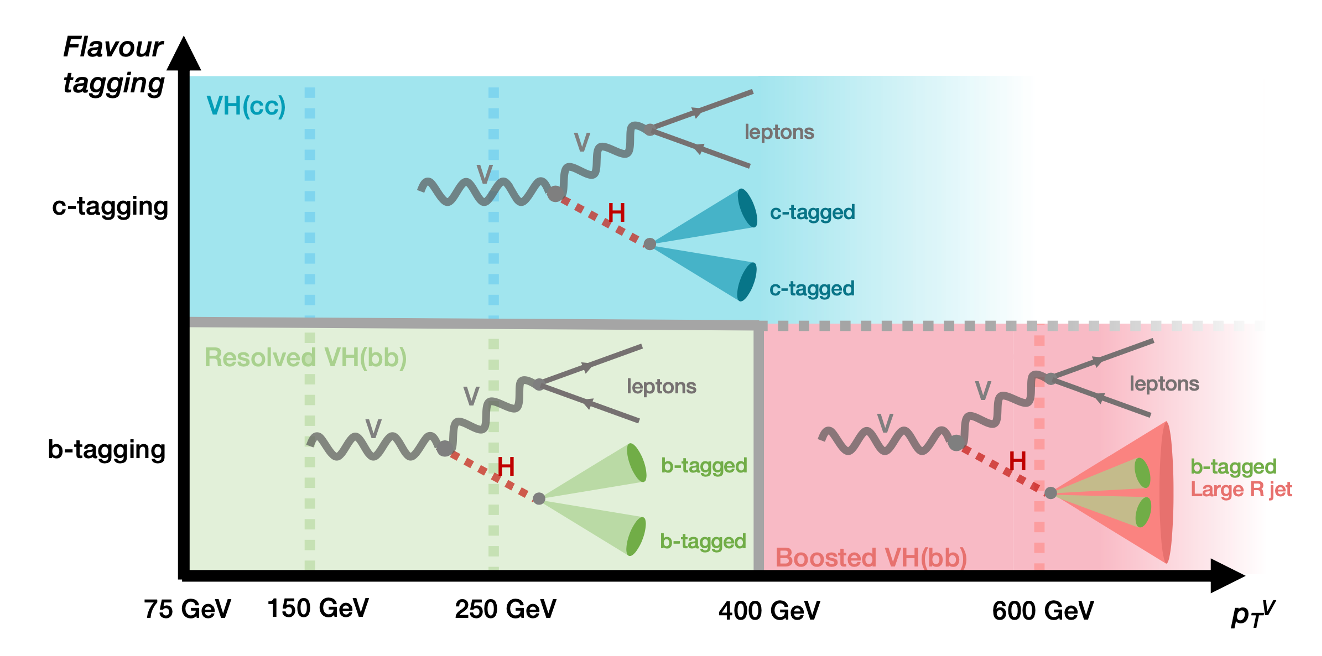
\includegraphics[width=\textwidth]{Images/VH/Cat/AnalysisRegime.png}
\caption{The analysis regimes considered in the combined $VH (H\rightarrow b\bar{b}/c\bar{c})$ analysis, from the internal documentation.} 
\label{fig:ana-strat}
\end{figure}

For each analysis region, three channels are defined based on the decay mode of the vector boson $V$: $Z \rightarrow \nu \nu$ defines the \textit{0-lepton} (0L), $W \rightarrow l \nu $ the \textit{1-lepton} (1L), and $Z \rightarrow l^+ l^-$ the \textit{2-lepton} (2L), where $l$ refers to an electron or a muon and $\nu$ to a neutrino. The signal considered are the  $VH (H\rightarrow b\bar{b})$ and $VH (H\rightarrow c\bar{c})$ processes, with the \gls{sm} diboson processes $VZ (Z\rightarrow b\bar{b})$ and $VZ (Z\rightarrow c\bar{c})$ considered as signals in a cross-check analysis. Having a larger cross-section and being kinematically similar to the signals, these processes can be measured with good statistical significance, thereby offering a suitable test case to verify the performance of the strategy deployed. The main backgrounds are the production of a vector boson with additional jets($V$+jets, mostly $Z$+jets in 0L and 2L, $W$+jets in 1L) and the top-quark processes (\textit{Top}, predominantly the top-quark pair production $t\bar{t}$, with one of the $t$ decaying leptonically, and a sub-leading contribution from single top-quark production with an extra $W$ boson, both in 0L and 1L). Minor backgrounds are the \gls{qcd} multi-jet\footnote{Thanks to the required presence of leptons in the final state.}, the single top process (without an extra associated $W$ boson) and non-signal diboson pair productions ($VV$). \\ 

Flavour tagging plays an essential role in the analysis, splitting the analysis phase space into different regimes of studies. The most important backgrounds are also split based on flavour components. The $V+$jets is split into three components: $V+$ heavy flavour jets ($V+$hf, including $V+bb$ and $V+cc$), $V+$ mixed flavour ($V+$mf, including the $V+bc$, $V+bl$, and $V+cl$), and the $V+$ light jet ($V+l$, including all other possible flavour selection including $\tau$'s). The top-quark background is also split by flavour: the Top(bb), in which the two selected jets are $b$-tagged, is treated separately from the Top(bbbq) which groups all other flavours as it is the dominant flavour background in $VH(H\rightarrow b\bar{b})$. \\

All backgrounds are simulated using \glsfirst{mc} simulation packages, except for the multi-jet which is estimated from a data-driven method\footnote{The top background in 2L is also estimated using data-driven techniques.} in the 1L channel and is negligible in other channels. To reproduce the conditions of the ATLAS detector, simulated samples are passed through the GEANT4 software \cite{Agostinelli:602040} and the ATLAS reconstruction software. The chapter is separated into different section introducing the datasets and simulation (Section \ref{sec-datasets}), a description of the reconstructed object (Section \ref{sec-obj}), the analysis selection and regimes (Section \ref{sec-regimeCat}), the event categorisation (Section \ref{sec-eventCat}), the modelling (Section \ref{sec-modelling}), the fit framework (Section \ref{sec-fitFramework}), and finally the main results (Section \ref{}).


\section{Data and Simulated Samples}\label{sec-datasets}
...

\section{Selection and Categorisation}\label{sec-selectionandcat}
\subsection{Object Selection}\label{sec-obj}
As introduced in Chapter \ref{chapter-ATLAS}, different types of information is collected by different sub-detectors of ATLAS. These must be combined to reconstruct physics objects. For the $VH (H\rightarrow c\bar{c})$ analysis, the reconstruction strategies of the most important objects are presented in this section. 

\paragraph{Primary Vertex:} events considered in the analysis are required to have at least one primary vertex reconstructed from tracks in the \gls{id} \cite{ATL-PHYS-PUB-2015-026}.

\paragraph{Electrons:} are reconstructed by matching a deposit in the EM calorimeter with a track in the \gls{id} \cite{Aaboud:2657964, Aad_2019}. Electrons are required to have a $p_T > 7$ GeV and $|\eta|<2.47$. They are identified with the \textit{loose} working point of a likelihood discriminant, matching the calorimeter shower shape and the track. The $e$ candidates must satisfy $p_T$-dependent isolation criteria in both the \gls{id} and calorimeter. In the 1L channel, the \textit{tight} likelihood criterion is used with stricter calorimeter isolation requirements to better reject the multi-jet background. The further requirements on the electron selection are lepton channel-dependent and summarised in Table~\ref{tbl:elOb}. %reference the electron segment earlier in the thesis.

\begin{table}[!htbp]
  \begin{center}
    \resizebox{0.99\textwidth}{!}{
      \begin{tabular}{ccccccc} \hline \hline
        Selection & $p_T$ & $\eta$ & ID & $d_{0}^{\mathrm sig}$ w.r.t. BL &  $|\Delta{z_{0}}\sin\theta|$ & Isolation \\ \hline
        VH-Loose & $>$7 GeV & $|\eta|< 2.47$ & \textit{Loose} & $ <5$ & $<0.5$ mm & Loose\_VarRad \\
        ZH-Signal & $>$27 GeV & $|\eta|< 2.47$ & \multicolumn{3}{c}{Same as VH-Loose} \\
        WH-Signal & \multicolumn{2}{c}{Same as ZH-Signal} & \textit{Tight} & \multicolumn{2}{c}{Same as ZH-Signal} & HighPtCaloOnly \\
        \hline\hline
      \end{tabular}
    }
    \caption{Electron Selection requirements.} % TODO Define BL and d0
    \label{tbl:elOb}
  \end{center}
\end{table}

A $VH$-Loose with loose likelihood identification is applied to electrons in all channels. Additionally, the $WH$-Signal and $ZH$-Signal criteria are applied in the 1L and 2L channels respectively, with a tighter $p_T$ due to the trigger threshold. The 1L likelihood identification and isolation selections are tighter to suppress the multi-jet background.

\paragraph{Muons:} are reconstructed by matching an energy deposit in the muon detector with information from the \gls{id} and \glsfirst{ms} \cite{Aad:2746302}. They are required to have a $p_T >$ 7 GeV, $|\eta| < 2.7$, to satisfy a \textit{loose} identification criteria and be isolated according to $p_T$ dependant criteria in the \gls{id}. Requirements are summarised in Table~\ref{tbl:muonOb} and vary depending on the lepton channel as for electrons. The $VH$-Loose requirement is applied to muons in all channels. The $WH$-Signal and $ZH$-Signal are additionally applied to the 1L and 2L channels respectively, with a stricter track-based isolation used in 1L.

\begin{table}[!htbp]
    \begin{center}
      \resizebox{0.99\textwidth}{!}{
        \begin{tabular}{ccccccc} \hline \hline
          Selection & $p_T$ & $\eta$ & ID & $d_{0}^{\mathrm sig}$ w.r.t. BL  & $|\Delta{z_{0}}\sin\theta|$ & Isolation \\ \hline
          VH-Loose & $>$7 GeV & $|\eta|< 2.7$ & Loose quality & $ <3$ & $<0.5$ mm & Loose\_VarRad \\
          ZH-Signal & $>$27 GeV & $|\eta| < 2.5$ & \multicolumn{4}{c}{Same as VH-Loose} \\
          %WH-Signal & $>$25 GeV ($>$27 when $p_T^V<$ 150 GeV) & $|\eta|< 2.5$ & Medium quality & $ <3$ & $<0.5$ mm & HighPtTrackOnly \\
          WH-Signal & \makecell[c]{$>$25 GeV if $p_T^V>$ 150 GeV\\ $>$27 GeV if $p_T^V<$ 150 GeV} & $|\eta|< 2.5$ & Medium quality & $ <3$ & $<0.5$ mm & HighPtTrackOnly \\
          \hline\hline
        \end{tabular}
      }
      \caption{Muon Selection requirements.} % TODO Define BL and d0
      \label{tbl:muonOb}
    \end{center}
  \end{table}
  
\paragraph{Taus:} hadronically decaying $\tau$-leptons are identified and vetoed in 1L using an \gls{rnn}-based tagger \cite{ATL-PHYS-PUB-2019-033}. Taus are required to have a $p_T >$ 20 GeV, $|eta| <$ 2.5, and to have 1 or 3 associated tracks. In 0L and 2L, if the jet passes a \textit{loose} working point requirement for hadronically decaying $\tau$-leptons, it is no longer considered as a jet and cannot be considered as a candidate for reconstruction of the Higgs boson. % TODO find more info from the object notes. % TODO also clarify this last thing about inclusive of tau events.

\paragraph{Missing Transverse Energy:} neutrinos are not detectable in ATLAS and their presence is inferred from momentum imbalance in the transverse plane to the beam axis. $E_T^{\textrm{miss}}$, also called MET, is the negative vectorial sum of the transverse momentum of physics objects\footnote{Electrons, muons, hadronic $\tau$, and jets.} and a track-based \textit{soft term}, to include a contribution from good quality tracks associated with the \glsfirst{pv} but not with any reconstructed physics object \cite{ATLASmetReco}. % TODO This citation is from the VHcc, check in object note it's still relevant.

\paragraph{Jets:} the analysis uses 3 types of jets, reconstructed with the anti-$k_t$ algorithm \cite{Cacciari:2008gp}:
\begin{enumerate}
  \item Small-$R$ jets: are reconstructed from topological clusters of energy deposit in the calorimeter based on the PFlow objects with a radius $R = 0.4$. Used in the resolved regime to reconstruct the Higgs candidate. A jet is considered as \textit{central} if $|\eta| < 2.5$ and $p_T$ > 20 GeV, and as \textit{forward} if 2.5 $\leq |\eta|$ < 4.5 and $p_T > 30$ GeV. Central (forward) jets with a $p_T < 60$ GeV ($p_T < 120$ GeV) are required to originate for the primary vertex as identified by the jet vertex tagger (\gls{jvt}) to limit the pile-up background \cite{atlasPUJVT}. \textit{Tight} jet cleaning criteria are applied to suppress non-collision background. % TODO more detail on jet cleaning criteria.
  \item Large-$R$ jets: are similar to small-$R$ jets with a larger radius $R = 1.0$, and required to have a $p_T > 250$ GeV and $|\eta| < 2$. They are used in the boosted regime to reconstruct the Higgs candidate. 
  \item Variable-$R$ (\gls{vr}) track-jets: are reconstructed with a $p_T$-dependent radius, optimised for double $b$-labelling efficiency of the boosted $H \rightarrow b\bar{b}$ decays \cite{ATL-PHYS-PUB-2017-010}. They are required to have a $p_T > 10$ GeV and $|\eta| < 2.5$. These track-jets are used to reconstruct the $b$-tagged objects inside the large-$R$ jet and for the boosted top-enriched \gls{cr}. 
\end{enumerate}
%TODO missing all of the corrections 

\paragraph{Flavour Tagging:} Jet flavour tagging is perhaps the most important part of the object reconstruction. The latest available Run 2 \gls{dl1r} tagger is used in the analysis for both $b$- and $c$-tagging in the resolved and boosted regime \cite{atlas:FTAGRUN2}. The methodology differs slightly between the two regimes of the analysis due to the different flavour tagging needs: 
\begin{itemize}
  \item In the resolved \vhb and \vhc, \gls{dl1r} is used to tag both $b$- and $c$-jets. The so-called \glsfirst{pcft} scheme, illustrated in Figure~\ref{fig:pseudotag}, is deployed to allow for a coherent joint definition and simultaneous calibration of $b$- and $c$-tagged jets, adopting the technique first introduced for 2D $c$-tagging in the \vhc \cite{Collaboration:2721696}. The \gls{dl1r} tagger assigns a $b$-score and a $c$-score to every selected jets. To tag a jet, the associated score must be higher than a specific cutoff value, defined to give a specific selection efficiency in simulated data, also known as a \glsfirst{wp}. From this score, the jet is assigned one of 4 possible labels, base on 2 $b$-tagging \gls{wp} and 2 $c$-tagging \gls{wp} tested in strict successive order. First a 60\% tight $b$-tagging working point (bin 4) is tested, followed by a looser 70\% $b$-\gls{wp} (bin 3). A jet passing these selections is labelled $B$\footnote{The difference between the $b$-tagged bins 3 and 4 is used in the discriminant \gls{bdt} of the analysis}. Otherwise, it is considered for $c$-tagging with first a \textit{tight} working point at 20\% efficiency (bin 2), followed by a \textit{loose} \gls{wp} at an exclusive efficiency of 20\% (bin 1) on the remaining jets - so that 40\% of $c$-jets are effectively selected in the combined tight and loose bins. A jet selected by the tight $c$-tagging \gls{wp} is labelled $T$, and $L$ if it passes the loose \gls{wp}. A jet failing to pass all \gls{wp}s is not tagged and labelled $N$ (bin 0). The $b$-tagging \gls{wp}s are official ATLAS ones for \gls{dl1r}, while those for $c$-tagging are optimised for the purpose of the analysis. The tagging efficiency of each bin is displayed in Table~\ref{tbl:PCFTtageff} displayed the tagging of each bin for the main flavours and $\tau$-leptons.
  \begin{table}[h!]
    \begin{center}
        \begin{tabular}{c|c|cccc}
          \hline \hline
          \multirow{2}{*}{PCFT bin} & \multirow{2}{*}{PCFT bin name} & \multicolumn{4}{c}{Jet tagging efficiency $\epsilon_{jet}$}\\
          & & $b$-jet &  $c$-jet &  light-jet & $\tau$-jet \\ 
          \hline
          1 & $c$-loose & 11.5\% & 20.5\% & 6.5\%   & 18.5\%\\
          2 & $c$-tight & 4.8\%  & 24.2\% & 0.9\%   & 19.5\%\\
          3 & $b$-70\%  & 11.2\% &  5.2\% & 0.13\%  &  1.7\%\\
          4 & $b$-60\%  & 58\%   & 2.65\% & 0.051\% & 0.49\%\\
          \hline \hline
        \end{tabular}
      \caption{Jet tagging efficiency for $b$-jet, $c$-jet, light-jet and $\tau$-jet in the \gls{pcft} bins, measured from a PowhegPythia8 simulated sample of semi-leptonic \ttb events, from the internal documentation.}
     \label{tbl:PCFTtageff}
    \end{center}
  \end{table}

  The calibration of all five bins of Figure~\ref{fig:pseudotag} was performed simultaneously for the analysis following the methodology described in Ref \cite{atlas:FTAGRUN2}, with some results presented in Appendix \ref{appsec-vh-ftagcal}.
  
  \begin{figure}[h!]
    \center
      \begin{minipage}[c]{0.69\textwidth}
        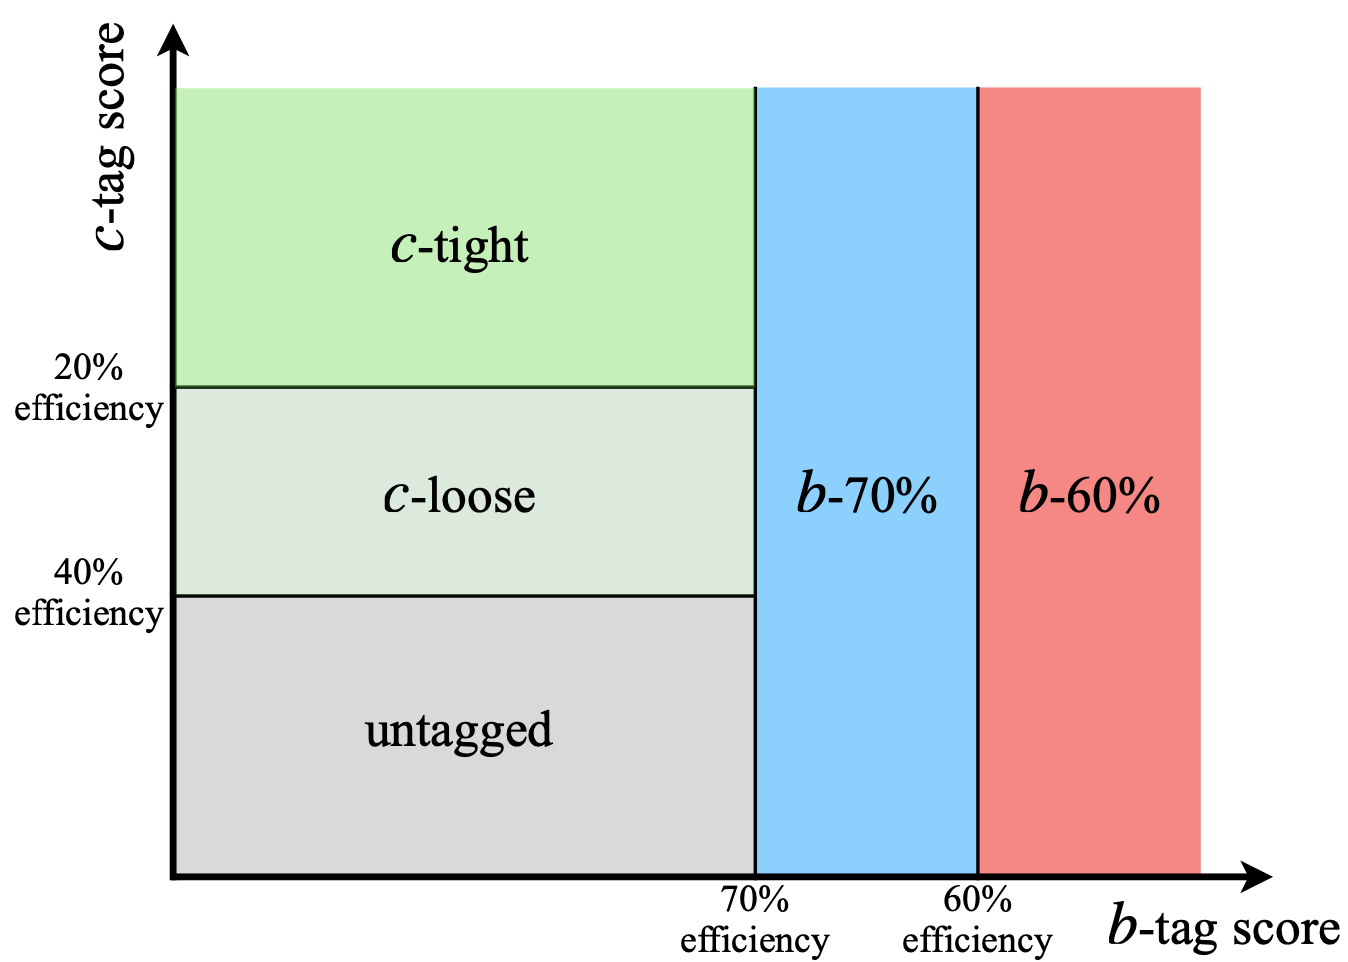
\includegraphics[width=0.98\textwidth]{Images/VH/pseudocontinuous.png}
      \end{minipage}
      \begin{minipage}[c]{0.3\textwidth}
        \caption{The \glsfirst{pcft} scheme used to simultaneously define 2 $b$-tagged, a tight $c$-tagged, a loose $c$-tagged, and a non-tagged bins, from the internal documentation. } 
        \label{fig:pseudotag}
      \end{minipage}
  \end{figure}
  \item The boosted regime only targets $b$-jets, following the single-purpose tagging used in the standard calibration of the tagger. As such, the standard pseudo-continuous $b$-tagging method is used. The track-jets associated to the leading large-$R$ jet are given a $b$-score based on the per-flavour probabilities outputted by \gls{dl1r}. The 85\% working point is adopted to maximise the signal yield, due to the important statistical limitations in the boosted regime. Track-jets passing this working point are $B$-tagged, otherwise they are untagged $N$. Studies showed that the very loose \gls{dl1r} \gls{wp} gives a better expected statistical significance than the then-available $X_{bb}$ tagger. The official calibration from Ref \cite{atlas:FTAGRUN2} is used, and extended to higher $p_T$ due to the wide range of $p_T$ probed in the analysis using uncertainty extrapolation, as presented in Appendix \ref{appsec-vh-ftagcal}.
\end{itemize}
While the analysis was underway, the superior single-jet \gls{gnn} taggers and the boosted objects $GN2X$ tagger introduced in Chapter \ref{chap-ftag} were not yet available as their calibration was an ongoing effort. Furthermore, switching to these new taggers was not feasible from a practical point of view in the timing of the analysis. They represent, however, an exciting avenue for progress in future iterations of this search, in both the resolved and boosted regimes. \\ % TODO check how the wp are defined %TODO also check the fc alue

\paragraph{Object Overlap:} overlap removal is applied to avoid double-counting electrons, muons, small-$R$ and large-$R$ jets, and hadronically decaying $\tau$'s that pass the object selection.